% Important: If latex complains about unicode characters,
% please use "\usepackage[utf8x]{inputenc}" in your preamble
% You can change the size of the picture by putting it into the construct:
% 1) \resizebox{10cm}{!}{"below picture"} to scale horizontally to 10 cm
% 2) \resizebox{!}{15cm}{"below picture"} to scale vertically to 15 cm
% 3) \resizebox{10cm}{15cm}{"below picture"} a combination of above two
% It is not recomended to use the scale option of the tikzpicture environment.
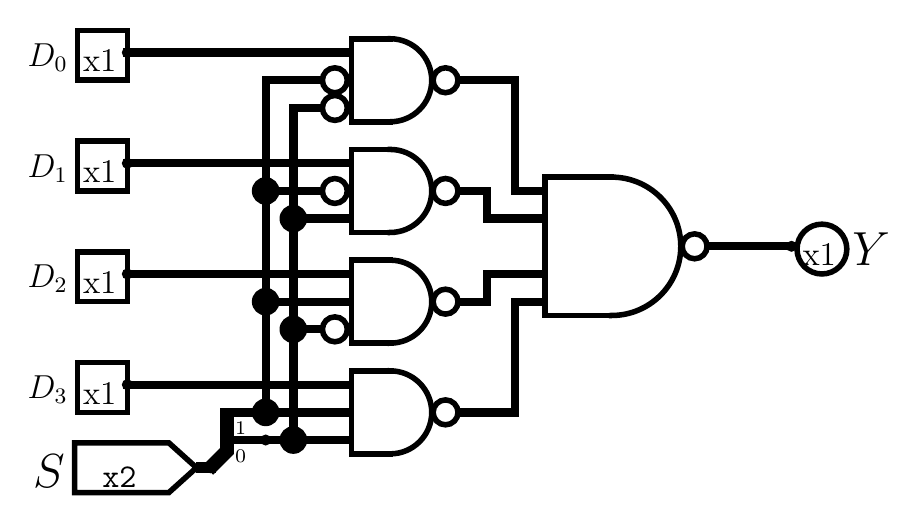
\begin{tikzpicture}[x=1pt,y=-1pt,line cap=rect]
\def\logisimfontA#1{\fontfamily{cmr}{#1}} % Replaced by logisim, original font was "SansSerif"
\def\logisimfontB#1{\fontfamily{cmtt}{#1}} % Replaced by logisim, original font was "Monospaced"
\def\logisimfontC#1{\fontfamily{Microsoft Sans Serif}{#1}}
\definecolor{custcol_0_0_0}{RGB}{0, 0, 0}
\definecolor{custcol_ff_ff_ff}{RGB}{255, 255, 255}
\draw [line width=3.0pt, custcol_0_0_0 ]  (276.0,87.0) -- (306.0,87.0) ;
\draw [line width=3.0pt, custcol_0_0_0 ]  (116.0,107.0) -- (116.0,147.0) -- (146.0,147.0) ;
\draw [line width=3.0pt, custcol_0_0_0 ]  (146.0,107.0) -- (116.0,107.0) -- (116.0,67.0) -- (116.0,27.0) -- (136.0,27.0) ;
\draw [line width=3.0pt, custcol_0_0_0 ]  (116.0,67.0) -- (136.0,67.0) ;
\draw [line width=3.0pt, custcol_0_0_0 ]  (126.0,77.0) -- (146.0,77.0) ;
\draw [line width=3.0pt, custcol_0_0_0 ]  (66.0,17.0) -- (146.0,17.0) ;
\draw [line width=3.0pt, custcol_0_0_0 ]  (186.0,67.0) -- (196.0,67.0) -- (196.0,77.0) -- (216.0,77.0) ;
\draw [line width=3.0pt, custcol_0_0_0 ]  (186.0,107.0) -- (196.0,107.0) -- (196.0,97.0) -- (216.0,97.0) ;
\draw [line width=3.0pt, custcol_0_0_0 ]  (66.0,57.0) -- (146.0,57.0) ;
\draw [line width=3.0pt, custcol_0_0_0 ]  (66.0,97.0) -- (146.0,97.0) ;
\draw [line width=3.0pt, custcol_0_0_0 ]  (66.0,137.0) -- (146.0,137.0) ;
\draw [line width=3.0pt, custcol_0_0_0 ]  (186.0,27.0) -- (206.0,27.0) -- (206.0,67.0) -- (216.0,67.0) ;
\draw [line width=3.0pt, custcol_0_0_0 ]  (186.0,147.0) -- (206.0,147.0) -- (206.0,107.0) -- (216.0,107.0) ;
\draw [line width=3.0pt, custcol_0_0_0 ]  (146.0,157.0) -- (126.0,157.0) -- (126.0,117.0) -- (126.0,77.0) -- (126.0,37.0) -- (136.0,37.0) ;
\draw [line width=3.0pt, custcol_0_0_0 ]  (126.0,117.0) -- (136.0,117.0) ;
\fill [line width=3.0pt, custcol_0_0_0]  (116.0,107.0) ellipse (5.0 and 5.0 );
\fill [line width=3.0pt, custcol_0_0_0]  (126.0,117.0) ellipse (5.0 and 5.0 );
\fill [line width=3.0pt, custcol_0_0_0]  (116.0,67.0) ellipse (5.0 and 5.0 );
\fill [line width=3.0pt, custcol_0_0_0]  (126.0,77.0) ellipse (5.0 and 5.0 );
\fill [line width=3.0pt, custcol_0_0_0]  (116.0,147.0) ellipse (5.0 and 5.0 );
\fill [line width=3.0pt, custcol_0_0_0]  (126.0,157.0) ellipse (5.0 and 5.0 );
\draw [line width=2.0pt, custcol_0_0_0 ]  (48.0,9.0) -- (65.0,9.0) ;
\draw [line width=2.0pt, custcol_0_0_0 ]  (66.0,9.0) -- (66.0,26.0) ;
\draw [line width=2.0pt, custcol_0_0_0 ]  (66.0,27.0) -- (49.0,27.0) ;
\draw [line width=2.0pt, custcol_0_0_0 ]  (48.0,27.0) -- (48.0,10.0) ;
\logisimfontA{\fontsize{12pt}{12pt}\selectfont\node[inner sep=0, outer sep=0, custcol_0_0_0, anchor=base west] at  (50.0,24.0)  {x1};}
\fill [line width=2.0pt, custcol_0_0_0]  (66.0,17.0) ellipse (2.0 and 2.0 );
\draw [line width=2.0pt, custcol_0_0_0 ]  (48.0,49.0) -- (65.0,49.0) ;
\draw [line width=2.0pt, custcol_0_0_0 ]  (66.0,49.0) -- (66.0,66.0) ;
\draw [line width=2.0pt, custcol_0_0_0 ]  (66.0,67.0) -- (49.0,67.0) ;
\draw [line width=2.0pt, custcol_0_0_0 ]  (48.0,67.0) -- (48.0,50.0) ;
\logisimfontA{\fontsize{12pt}{12pt}\selectfont\node[inner sep=0, outer sep=0, custcol_0_0_0, anchor=base west] at  (50.0,64.0)  {x1};}
\fill [line width=2.0pt, custcol_0_0_0]  (66.0,57.0) ellipse (2.0 and 2.0 );
\draw [line width=2.0pt, custcol_0_0_0 ]  (48.0,89.0) -- (65.0,89.0) ;
\draw [line width=2.0pt, custcol_0_0_0 ]  (66.0,89.0) -- (66.0,106.0) ;
\draw [line width=2.0pt, custcol_0_0_0 ]  (66.0,107.0) -- (49.0,107.0) ;
\draw [line width=2.0pt, custcol_0_0_0 ]  (48.0,107.0) -- (48.0,90.0) ;
\logisimfontA{\fontsize{12pt}{12pt}\selectfont\node[inner sep=0, outer sep=0, custcol_0_0_0, anchor=base west] at  (50.0,104.0)  {x1};}
\fill [line width=2.0pt, custcol_0_0_0]  (66.0,97.0) ellipse (2.0 and 2.0 );
\draw [line width=2.0pt, custcol_0_0_0 ]  (48.0,129.0) -- (65.0,129.0) ;
\draw [line width=2.0pt, custcol_0_0_0 ]  (66.0,129.0) -- (66.0,146.0) ;
\draw [line width=2.0pt, custcol_0_0_0 ]  (66.0,147.0) -- (49.0,147.0) ;
\draw [line width=2.0pt, custcol_0_0_0 ]  (48.0,147.0) -- (48.0,130.0) ;
\logisimfontA{\fontsize{12pt}{12pt}\selectfont\node[inner sep=0, outer sep=0, custcol_0_0_0, anchor=base west] at  (50.0,144.0)  {x1};}
\fill [line width=2.0pt, custcol_0_0_0]  (66.0,137.0) ellipse (2.0 and 2.0 );
\draw [line width=4.0pt, custcol_0_0_0 ]  (93.0,167.0) -- (96.0,167.0) ;
\draw [line width=2.0pt, custcol_0_0_0 ]  (81.0,176.0) -- (91.0,167.0) -- (81.0,158.0) -- (47.0,158.0) -- (47.0,176.0) -- cycle;
\logisimfontB{\fontsize{12pt}{12pt}\selectfont\node[inner sep=0, outer sep=0, custcol_0_0_0, anchor=base west] at  (57.0,174.0)  {x2};}
\logisimfontC{\fontsize{16pt}{16pt}\fontseries{bx}\selectfont\node[inner sep=0, outer sep=0, custcol_0_0_0, anchor=base west] at  (32.0,174.0)  {$S$};}
\fill [line width=2.0pt, custcol_0_0_0]  (96.0,167.0) ellipse (2.0 and 2.0 );
\draw [line width=3.0pt, custcol_0_0_0 ]  (106.0,147.0) -- (116.0,147.0) -- (102.0,147.0) ;
\draw [line width=3.0pt, custcol_0_0_0 ]  (126.0,157.0) -- (116.0,157.0) -- (102.0,157.0) ;
\draw [line width=5.0pt, custcol_0_0_0 ]  (102.0,148.0) -- (102.0,161.0) -- (97.0,166.0) ;
\logisimfontA{\fontsize{7pt}{7pt}\selectfont\node[inner sep=0, outer sep=0, custcol_0_0_0, anchor=base west] at  (105.0,155.0)  {1};}
\logisimfontA{\fontsize{7pt}{7pt}\selectfont\node[inner sep=0, outer sep=0, custcol_0_0_0, anchor=base west] at  (105.0,165.0)  {0};}
\fill [line width=5.0pt, custcol_0_0_0]  (96.0,167.0) ellipse (2.0 and 2.0 );
\fill [line width=5.0pt, custcol_0_0_0]  (116.0,147.0) ellipse (2.0 and 2.0 );
\fill [line width=5.0pt, custcol_0_0_0]  (116.0,157.0) ellipse (2.0 and 2.0 );
\draw [line width=2.0pt, custcol_0_0_0]  (317.0,88.0) ellipse (9.0 and 9.0 );
\logisimfontA{\fontsize{12pt}{12pt}\selectfont\node[inner sep=0, outer sep=0, custcol_0_0_0, anchor=base west] at  (310.0,94.0)  {x1};}
\logisimfontC{\fontsize{16pt}{16pt}\fontseries{bx}\selectfont\node[inner sep=0, outer sep=0, custcol_0_0_0, anchor=base west] at  (328.0,94.0)  {$Y$};}
\fill [line width=2.0pt, custcol_0_0_0]  (306.0,87.0) ellipse (2.0 and 2.0 );
\draw [line width=2.0pt, custcol_0_0_0]  (141.0,27.0) ellipse (4.5 and 4.5 );
\draw [line width=2.0pt, custcol_0_0_0]  (141.0,37.0) ellipse (4.5 and 4.5 );
\draw [line width=2.0pt, custcol_0_0_0] (161.0,42.0) arc (90.0:-90.0:15.0 and 15.0 );
\draw [line width=2.0pt, custcol_0_0_0 ]  (161.0,12.0) -- (147.0,12.0) -- (147.0,42.0) -- (161.0,42.0) ;
\draw [line width=2.0pt, custcol_0_0_0]  (181.0,27.0) ellipse (4.5 and 4.5 );
\draw [line width=2.0pt, custcol_0_0_0]  (141.0,67.0) ellipse (4.5 and 4.5 );
\draw [line width=2.0pt, custcol_0_0_0] (161.0,82.0) arc (90.0:-90.0:15.0 and 15.0 );
\draw [line width=2.0pt, custcol_0_0_0 ]  (161.0,52.0) -- (147.0,52.0) -- (147.0,82.0) -- (161.0,82.0) ;
\draw [line width=2.0pt, custcol_0_0_0]  (181.0,67.0) ellipse (4.5 and 4.5 );
\draw [line width=2.0pt, custcol_0_0_0]  (141.0,117.0) ellipse (4.5 and 4.5 );
\draw [line width=2.0pt, custcol_0_0_0] (161.0,122.0) arc (90.0:-90.0:15.0 and 15.0 );
\draw [line width=2.0pt, custcol_0_0_0 ]  (161.0,92.0) -- (147.0,92.0) -- (147.0,122.0) -- (161.0,122.0) ;
\draw [line width=2.0pt, custcol_0_0_0]  (181.0,107.0) ellipse (4.5 and 4.5 );
\draw [line width=2.0pt, custcol_0_0_0] (161.0,162.0) arc (90.0:-90.0:15.0 and 15.0 );
\draw [line width=2.0pt, custcol_0_0_0 ]  (161.0,132.0) -- (147.0,132.0) -- (147.0,162.0) -- (161.0,162.0) ;
\draw [line width=2.0pt, custcol_0_0_0]  (181.0,147.0) ellipse (4.5 and 4.5 );
\draw [line width=2.0pt, custcol_0_0_0] (241.0,112.0) arc (90.0:-90.0:25.0 and 25.0 );
\draw [line width=2.0pt, custcol_0_0_0 ]  (241.0,62.0) -- (217.0,62.0) -- (217.0,112.0) -- (241.0,112.0) ;
\draw [line width=2.0pt, custcol_0_0_0]  (271.0,87.0) ellipse (4.5 and 4.5 );
\logisimfontA{\fontsize{12pt}{12pt}\selectfont\node[inner sep=0, outer sep=0, custcol_0_0_0, anchor=base west] at  (30.0,62.0)  {$D_1$};}
\logisimfontA{\fontsize{12pt}{12pt}\selectfont\node[inner sep=0, outer sep=0, custcol_0_0_0, anchor=base west] at  (30.0,102.0)  {$D_2$};}
\logisimfontA{\fontsize{12pt}{12pt}\selectfont\node[inner sep=0, outer sep=0, custcol_0_0_0, anchor=base west] at  (30.0,142.0)  {$D_3$};}
\logisimfontA{\fontsize{12pt}{12pt}\selectfont\node[inner sep=0, outer sep=0, custcol_0_0_0, anchor=base west] at  (30.0,22.0)  {$D_0$};}
\end{tikzpicture}

